\hypertarget{ux562ux561ux576-ux562-ux583ux578ux583ux578ux56dux561ux56fux561ux576ux576ux565ux580}{%
\section{Բան Բ․
Փոփոխականներ}\label{ux562ux561ux576-ux562-ux583ux578ux583ux578ux56dux561ux56fux561ux576ux576ux565ux580}}

\begin{quote}
\emph{Փոփոխականների հայտարաումը, փոփոխականի տիպը, փոփոխականին արժեքի
վերագրումը, փոփոխականի հասցե, ներմուծման ստանդարտ հոսքից տվյալների
կարդալը։}
\end{quote}

C լեզվով գրված ամեն մի ծրագիր, բացառությամբ պարզագույն դեպքերի,
պարունակում է փոփոխականներ։ \emph{Փոփոխականը} մի օբյեկտ է, որը ծրագրի
կատարման տարբեր պահերի կարող է պարունակել նախապես որոշված արժեքների
տիրույթի (domain) մի որևէ արժեք։ Յուրաքանչյուր փոփոխական, որ հանդիպում է
ծրագրում, պետք է նախապես \emph{սահմանված} լինի։ Փոփոխականի սահմանումը
բաղկացած է նրա \emph{տիպը} որոշող ծառայողական բառից և փոփոխականի
\emph{անունից}։ Օրինակ,

\begin{Shaded}
\begin{Highlighting}[]
\DataTypeTok{double}\NormalTok{ a;      }\CommentTok{/* a{-}ն կրկնակի ճշտությամբ իրական թիվ է */}
\DataTypeTok{float}\NormalTok{ b, c;    }\CommentTok{/* b{-}ն և c{-}ն սովորական ճշտության իրական թվեր են */}
\DataTypeTok{int}\NormalTok{ d0, d1;    }\CommentTok{/* d0{-}ն և d1{-}ը ամբողջ թվեր են */}
\DataTypeTok{char}\NormalTok{ sym;      }\CommentTok{/* sym{-}ը նիշ է (character) */}
\DataTypeTok{long} \DataTypeTok{int}\NormalTok{ e1a;  }\CommentTok{/* e1a{-}ն երկար ամբողջ թիվ է */}
\end{Highlighting}
\end{Shaded}

Այստեղ \texttt{double}, \texttt{float}, \texttt{int}, \texttt{char} և
\texttt{long} բառերը \emph{ծառայողական բառեր} են և \emph{ներդրված}
տիպերի անուններ։ Իսկ \texttt{a}, \texttt{b}, \texttt{c}, \texttt{d0},
\texttt{d1}, \texttt{sym} և \texttt{e1a} բառերը իդենտիֆիկատորներ են։ C
լեզվի \emph{իդենտիֆիկատորը} տառով կամ ընդգծման նիշով՝ «\texttt{\_}»,
սկսվող տառերի ու թվանշանների հաջորդականություն է։ Պետք է հիշել, որ C
լեզվում մեծատառերն ու փոքրատառերը տարբերվում են, այսինքն՝ \texttt{abc0}
և \texttt{aBc0} բառերը տարբեր իդենտիֆիկատորներ են։

Փոփոխականի տիպով որոշվում է հիշողությունում նրա զբաղեցրած բայթերի քանակը
և նրա հետ կատարվող թույլատրելի գործողությունները։ Օրինակ, իմ համակարգում
\texttt{int} տիպ ունեցող փոփոխականը զբաղեցնում է 4 բայթ, \texttt{double}
տիպ ունեցող փոփոխականը՝ 8 բայթ, իսկ \texttt{char} տիպի փոփոխականը՝ 1
բայթ։ Ծրագրի կատարման ժամանակ փոփոխականի զբողեցրած հիշողության չափը
կարելի է ստանալ \texttt{sizeof} գործողության օգնությամբ։ Օրինակ, եթե
\texttt{a0}-ն \texttt{double} տիպի փոփոխական է, ապա \texttt{sizeof(a0)}
արտհայտության արժեքը 8 է։ \texttt{sizeof} գործողության արգումենտը կարող
է լինել ոչ միայն փոփոխականի անուն, այլ նաև C լեզվի տիպի անուն։ Օրինակ,
\texttt{sizeof(unsigned\ int)} արտահայտության արժեքը առանց նշանի ամբողջ
թվերը որոշող տիպի չափն է։

Փոփոխականին կարելի է արժեք վերագրել հենց անմիջապես հայտարարության
ժամանակ։ Ընդհանրապես, ծրագրավորման «լավ ոճ» է համարվում, երբ փոփոխականին
արժեք է վերագրվում հայտարարության հետ միասին։ Օրինակ․

\begin{Shaded}
\begin{Highlighting}[]
\DataTypeTok{int}\NormalTok{ count = }\DecValTok{0}\NormalTok{;       }\CommentTok{/* հայտարարել count ամբողջաթիվ փոփոխականը՝ 0 արժեքով */}
\DataTypeTok{double}\NormalTok{ pi = }\FloatTok{3.1415}\NormalTok{;  }\CommentTok{/* հայտարարել pi իրական փոփոխականը՝ 3.1415 արժեքով */}
\DataTypeTok{char}\NormalTok{ c = }\CharTok{\textquotesingle{}A\textquotesingle{}}\NormalTok{;        }\CommentTok{/* հայտարարել c նիշային փոփոխականը՝ «A» արժեքով */}
\end{Highlighting}
\end{Shaded}

Փոփոխականին նոր արժեք է տրվում \texttt{=} \emph{վերագրման}
գործողությամբ։ Օրինակ,

\begin{Shaded}
\begin{Highlighting}[]
\DataTypeTok{double}\NormalTok{ a0, a1, b0;  }\CommentTok{/* a0{-}ն, a1{-}ը և b0{-}ն իրական թվեր են */}
\NormalTok{a0 = }\FloatTok{2.36}\NormalTok{;          }\CommentTok{/* a0{-}ին վերագրել 2.36 */}
\NormalTok{a1 = }\FloatTok{4.1}\NormalTok{;           }\CommentTok{/* a1{-}ին վերագրել 4.1 */}
\NormalTok{b0 = a0 + a1;       }\CommentTok{/* b0{-}ին վերագրել a0{-}ի և a1{-}ի գումարը */}
\end{Highlighting}
\end{Shaded}

Ծրագրի կատարման ժամանակ ամեն մի հայտարարված փոփոխականի հատկացվում է
հիշողության մի որոշակի տիրույթ։ Այդ տիրույթի առաջին բայթի համարը
փոփոխականի \emph{հասցեն} է, որը կարող ենք ստանալ \texttt{\&} միտեղանի
(unary) գործողությամբ։ Օրինակ, \texttt{\&pi} արտհայտության արժեքը
\texttt{pi} փոփոխականի հասցեն է։

Ես ուզում եմ ցույց տալ ու մեկնաբանել մի ծրագիր, որն օգտագործողից
պահանջում է ներմուծել հարթության մի որևէ կետի դեկարտյան կոորդինատները և
արտածում է նույն այդ կետի բևեռային կոորդինատները։

Պարզ է, որ կետի դեկարտյան կոորդինատները ներկայացնելու համար պետք է
հայտարարել \texttt{x} և \texttt{y} իրական փոփոխականները, ապա դրանց
արժեքները կարդալ ստեղնաշարից։

\begin{Shaded}
\begin{Highlighting}[]
\DataTypeTok{double}\NormalTok{ x = }\FloatTok{0.0}\NormalTok{, y = }\FloatTok{0.0}\NormalTok{;}
\NormalTok{scanf( }\StringTok{"\%lf"}\NormalTok{, \&x );  }\CommentTok{/* կարդալ իրական թիվ և վերագրել x{-}ին */}
\NormalTok{scanf( }\StringTok{"\%lf"}\NormalTok{, \&y );  }\CommentTok{/* նույնը՝ y{-}ի համար */}
\end{Highlighting}
\end{Shaded}

C լեզվի ստանդարտ գրադարանի \texttt{scanf} (scan formated ― ֆորմատավորված
ընթերցում) ֆունկցիան ներմուծման ստանդարտ հոսքից (stdin) կարդում է նիշերի
հաջորդականություն և այն ձևափոխում է ըստ տրված ֆորմատի։ \texttt{scanf}
ֆունկցիայի առաջին արգումենտը ֆորմատավորման տողն է, որ կարող է պարունակել
\texttt{\%} նիշով սկսվող ֆորմատավորման հրահանգներ։ \texttt{\%} նիշին
հաջորդող նիշերով որոշվում է, թե ինչպես պետք է մեկնաբանվեն կարդացած
տվյալները։ Օրինակ, եթե գրված է \texttt{\%d}, ապա սա նշանակում է, որ
հոսքից կարդացած նիշերը պետք է դիտարկել որպես տասական (decimal) թիվ։ Եթե
գրված է \texttt{\%f}, ապա՝ սովորական ճշտության իրական (float) թիվ։
Ֆորմատավորման հրահանգներին համապատասխան ձևափոխված տվյալները գրվում են
\texttt{scanf} ֆունկցիայի երկրորդ և հաջորդ արգումենտներով տրված
հասցեներում։ Օրինակ.

\begin{Shaded}
\begin{Highlighting}[]
\NormalTok{scanf( }\StringTok{"\%lf"}\NormalTok{, \&x );}
\end{Highlighting}
\end{Shaded}

արտահայտության մեջ տրված \texttt{"\%lf"} ֆորմատը նշում է, որ պետք է
կարդալ երկար իրական թիվ (l - long, f - float) և կարդացած արժեքը գրել
\texttt{x} փոփոխականի զբաղեցրած հասցեում։ \texttt{scanf} ֆունկցիային
փոխանցվում է ոչ թե փոփոխականը, այլ նրա հասցեն՝ այն տեղը, որտեղ պետք է
գրել կարդացած և ֆորմատավորած տվյալները։

\texttt{scanf} և \texttt{printf} ֆունկցիաների ֆորմատավորման հրահանգների
մասին ես դեռ պատմելու շատ առիթներ կունենամ։ Առայժմ բավական է իմանալ, որ
\texttt{"\%lf"} ֆորմատը կարդում է \texttt{double} արժեք։

\texttt{x} և \texttt{y} փոփոխականների արժեքները կարդացող \texttt{scanf}
ֆունկցիայի երկու կանչերը կարելի է միավորել մեկի մեջ՝ \texttt{"\%lf"}
ֆորմատը փոխարինելով \texttt{"\%lf,\%lf"} ֆորմատով։ Սա նշանակում է, որ
\texttt{scanf} ֆունկցիան ստեղնաշարից կարդալու է իրարից ստորակետով
բաժանված երկու \texttt{double} արժեք։

\begin{Shaded}
\begin{Highlighting}[]
\DataTypeTok{double}\NormalTok{ x = }\FloatTok{0.0}\NormalTok{, y = }\FloatTok{0.0}\NormalTok{;}
\NormalTok{scanf( }\StringTok{"\%lf,\%lf"}\NormalTok{, \&x, \&y );  }\CommentTok{/* կարդալ երկու իրական թվեր և վերագրել x{-}ին ու y{-}ին */}
\end{Highlighting}
\end{Shaded}

Դե քանի որ \texttt{scanf} ֆունկցիայի ֆորմատավորման տողը պարունակում է
երկու ֆորմատավորման հրահանգ, ապա պետք է տալ կարդացած արժեքները գրելու
երկու տեղ՝ \texttt{\&x} և \texttt{\&y}։

Եթե պետք լինի օգտագործողին ստիպել, որ նա կետի կոորդինատները ներմուծի
\texttt{(} և \texttt{)} փակագծերի մեջ վերցրած, ապա կարելի է
ֆորմատավորման տողը գրել \texttt{"(\%lf,\%lf)"} տեսքով։ Բառացիորեն սա
կարելի է կարդալ հետևյալ կերպ. «\emph{կարդալ \texttt{(} նիշը, կարդալ
\texttt{double} թիվ, կարդալ \texttt{,} նիշը, կարդալ \texttt{double} թիվ,
կարդալ \texttt{)} նիշը}»։

Կետի \texttt{x} \emph{աբսցիսի} և \texttt{y} \emph{օրդինատի} արժեքները
կարդալուց հետո պետք է հաշվել նրա բևեռային կոորդինատները՝ \texttt{ρ}
\emph{շառավիղը} և \texttt{φ} \emph{ազիմուտը}։ Կոորդինատների բևեռային
համակարգում \texttt{ρ}-ն որոշվում է որպես կետի հեռավորությունն բևեռից,
իսկ \texttt{φ}-ն՝ որպես շառավղի և բևեռային առանցքի կազմած անկյուն։
Բևեռային շառավիղը որոշվում է Պյութագորասի թեորեմով՝ քանի որ այն իրենից
ներկայացնում է ուղղանկյուն եռանկյան ներքնաձիգ։ Բևեռային անկյունը
որոշելու համար էլ օգտվում ենք նույն ուղղանկյուն եռանկյունից և այն
փաստից, որ որոնելի անկյան տանգենսը հավասար է նրա դիմացի էջի երկարության
հարաբերությանը կից էջի երկարությանը՝ \texttt{y/x}, դե իսկ անկյան
մեծությունն էլ հավասար կլինի այդ վերջին հարաբերության արկտանգենսին։

\begin{figure}
\centering
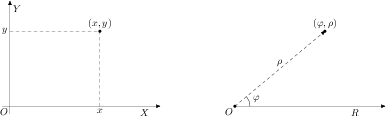
\includegraphics{nacl-fig-1.png}
\caption{կոորդինատներ}
\end{figure}

Ասվածը C լեզվով կարող եմ գրել հետևյալ արտահայտություններով․

\begin{Shaded}
\begin{Highlighting}[]
\DataTypeTok{double}\NormalTok{ rho = sqrt( x * x + y * y );}
\DataTypeTok{double}\NormalTok{ phi = atan2( y, x );}
\end{Highlighting}
\end{Shaded}

\texttt{sqrt} ֆունկցիան վերադարձնում է արգումենտի երկրորդ աստիճանի
արմատը, իսկ \texttt{atan2} ֆունկցիան վերադարձնում է \texttt{0} սկզբնակետ
և \texttt{(x,y)} վերջնակետ ունեցող վեկտորի և աբսցիցների առանցքի կազմած
անկյունը ռադիաններով։ Այս երկու ֆունկցիաներն էլ սահմանված են C լեզվի
ստանդարտ գրադարանի \texttt{math.h} ֆայլում։

\texttt{rho} և \texttt{phi} արժեքների հաշվարկից հետո պարզապես պետք է
արտածել դրանք․

\begin{Shaded}
\begin{Highlighting}[]
\NormalTok{puts( }\StringTok{"Բևեռային կոորդնատներն են․ "}\NormalTok{ );}
\NormalTok{printf( }\StringTok{"ρ = \%lf, φ = \%lf}\SpecialCharTok{\textbackslash{}n}\StringTok{"}\NormalTok{, rho, phi );}
\end{Highlighting}
\end{Shaded}

\texttt{printf} ֆունկցիայում նույնպես օգտագործվել են \texttt{"\%lf"}
ֆորմատավորման հրահանգները։ Քանի որ \texttt{printf} ֆունկցիան իր
արգումենտները չի փոխում, այստեղ նրան փոխանցում ենք \texttt{x} և
\texttt{y} փոփոխականների արժեքները, այլ ոչ թե հասցեները։

Վերջ։ Մնում է այս ամենը հավաքել \texttt{main} ֆունկցիայի մեջ,
կոմպիլյացնել, գործարկել ու տեսնել արդյունքները։ Ես ամբողջ ծրագիրը գրել
եմ \texttt{prog02.c} ֆայլի մեջ։

\begin{Shaded}
\begin{Highlighting}[]
\PreprocessorTok{\#include }\ImportTok{\textless{}stdio.h\textgreater{}}
\PreprocessorTok{\#include }\ImportTok{\textless{}math.h\textgreater{}}

\DataTypeTok{int}\NormalTok{ main()}
\NormalTok{\{}
  \DataTypeTok{double}\NormalTok{ x = }\FloatTok{0.0}\NormalTok{, y = }\FloatTok{0.0}\NormalTok{;}
\NormalTok{  puts( }\StringTok{"Ներմուծիր դեկարտյան կոորդինատները x,y․ "}\NormalTok{ );}
\NormalTok{  scanf( }\StringTok{"\%lf,\%lf"}\NormalTok{, \&x, \&y );}

  \DataTypeTok{double}\NormalTok{ rho = sqrt( x * x + y * y );}
  \DataTypeTok{double}\NormalTok{ phi = atan2( y, x );}

\NormalTok{  puts( }\StringTok{"Բևեռային կոորդնատներն են․ "}\NormalTok{ );}
\NormalTok{  printf( }\StringTok{"ρ = \%lf, φ = \%lf}\SpecialCharTok{\textbackslash{}n}\StringTok{"}\NormalTok{, rho, phi );}

  \ControlFlowTok{return} \DecValTok{0}\NormalTok{;}
\NormalTok{\}}
\end{Highlighting}
\end{Shaded}

\texttt{\#include} դիրեկտիվով կցվել են \texttt{stdio.h} և
\texttt{math.h} ֆայլերը։ Առաջինից օգտագործվում են \texttt{puts},
\texttt{scanf} և \texttt{printf} ֆունկցիաները, իսկ երկրորդից՝
\texttt{sqrt} և \texttt{atan2} ֆունկցիաները։

Երբ ես փորձում եմ \texttt{prog02.c} ֆայլը կոմպիլյացնել այնպես, ինչպես դա
արեցի առաջին զրույցում նկարագրված \texttt{prog01.c} ֆայլի հետ.

\begin{Shaded}
\begin{Highlighting}[]
\NormalTok{$ }\FunctionTok{clang}\NormalTok{ prog02.c {-}o prog2}
\end{Highlighting}
\end{Shaded}

ապա ստանում եմ մի հաղորդագրություն, որն ասում է, թե linker ծրագիրը՝
\emph{կապերի խմբագրիչը}, չի գտել \texttt{sqrt} և \texttt{atan2}
ֆունկցիաները։

\begin{verbatim}
/tmp/prog02-80b543.o: In function `main':
prog02.c:(.text+0x6a): undefined reference to `sqrt'
prog02.c:(.text+0x91): undefined reference to `atan2'
clang: error: linker command failed with exit code 1 (use -v to see invocation)
\end{verbatim}

Բանն այն է, որ \texttt{math.h} ֆայլը պարունակում է մաթեմատիկական
գրադարանի հայտարարությունները, բայց ոչ սահմանումները։ Սահմանումները,
այսինքն մաթեմատիկական գրադարանի կոմպիլյացված օբյեկտային կոդը, գտնվում է
\texttt{libm.a} (ստատիկ) և \texttt{libm.so} (դինամիկ) օբյեկտային
ֆայլերում։ ՈՒրեմն, երբ ծրագրի ֆայլում \texttt{\#include} դիրեկտիվով
կցում ենք \texttt{math.h} ֆայլը, դա անում ենք, պարզպես, որ կոմպլյատորն
իմանա օգտագործվող ֆունկցիաների հայտարարությունները։ Իսկ կապերի խմբագրման
(link) ժամանակ, երբ պետք է ստացվի կատարվող ֆայլ, կոմպիլյատորի
\texttt{-l} պարամետրով պիտի տալ \texttt{m} գրադարանը (գրադարանների
անունները սկսվում են lib նախածանցով, բայց \texttt{-l} պարամետրով
գրադարանը նշելիս lib-ը չի գրվում)։

\texttt{prog02.c} ֆայլի կոմպիլյացիայի՝ վերը բերված հրամանն իրականում
կատարվում է չորս քայլով՝ \emph{նախամշակում} (preprocessing),
\emph{կոմպիլյացիա} (compilation), \emph{ասեմբլացում} (assembly) և
\emph{կապակցում} (linking)։ Նախամշակման փուլում մշակվում են \texttt{\#}
նիշով սկսվող հրահանգները. \texttt{\#include} հրահանգով կցվում են ֆայլեր,
\texttt{\#define} հրահանգով սահմանվում են մակրոսներ և այլն (նախամշակման
քայլի մասին մանրամասն կխոսեմ քիչ ավելի ուշ)։ Կոմպիլյացիայի փուլում C
լեզվով գրված ծրագիրը թարգմանվում է ասեմբլերի լեզվով գրված ծրագրի։
Ասեմբլացման փուլում ասեմբլերի լեզվով ծրագիրը թարգմանվում է կոնկրետ
ապարատային պլատորմի վրա աշխատող կոնկրետ օպերացիոն համակարգի օբյեկտային
կոդի։ Կապակցման փուլում իրար են կցվում առանձին-առանձին կոմպիլյացված
օբյեկտային մոդուլները, ստեղծվում է կատարվող մոդուլ։ Եթե ուզում ես
տեսնել, թե այդ միջանկյալ քայլերում ինչ ֆայլեր են գեներացվում, ապա կարող
ես կոմպիլյացիայի հրամանին տալ \texttt{-\/-save-temps} պարամետրը.

\begin{Shaded}
\begin{Highlighting}[]
\NormalTok{$ }\FunctionTok{clang}\NormalTok{ {-}{-}save{-}temps {-}o prog02 prog02.c {-}lm}
\end{Highlighting}
\end{Shaded}

Այս հրամանի կատարումից հետո ստեղծվում են \texttt{prog02.i},
\texttt{prog02.s}, \texttt{prog02.o}, \texttt{prog02} ֆայլերը։ Դրանք
համապատասխանաբար նախամշակման, կոմպիլյացիայի և ասեմբլացման փուլերում
ստեղծված ֆայլերն են։ Կապակցման արդյունքում ստացված ֆայլը ստանում է
կոմպիլյատորի ՝-օ՝ պարամետրով տրված անունը։

Կոմպիլյացիայի քայլերը ես էլ կարող եմ առանձնացնել։

\begin{enumerate}
\def\labelenumi{\arabic{enumi}.}
\tightlist
\item
  \texttt{clang\ -E\ -o\ prog02.i\ prog02.c} ― Նախամշակել, բայց
  չկոմպիլյացնել։ Ստեղծվում է \texttt{prog02.i} ֆայլը։
\item
  \texttt{clang\ -S\ -o\ prog02.s\ prog02.i} ― Կոմպիլյացնել նախամշակված
  ֆայլը, բայց չասեմբլացնել։ Ստեղծվում է \texttt{prog02.s} ֆայլը։
\item
  \texttt{clang-3.5\ -c\ -o\ prog02.o\ prog02.s} ― Ասեմբլերային ֆայլը
  թարգմանել օբյեկտային ֆայլի։ Ստեղծվում է \texttt{prog02.o} ֆայլը։
\item
  \texttt{clang\ -o\ prog02\ prog02.o\ -lm} ― Օբյեկտային ֆայլը կապակցել
  գրադարանների հետ և ստեղծել \texttt{prog02} կատարվող մոդուլը։
\end{enumerate}

Հիմա արդեն ամեն ինչ կարգին է․ ֆայլը թարգմանվել է և կառուցվել է
\texttt{prog02} կատարվող ֆայլը։ Գործարկեմ այն ու տեսնեմ, թե ինչ է
ստացվում․

\begin{Shaded}
\begin{Highlighting}[]
\NormalTok{$ }\ExtensionTok{./prog02}
\NormalTok{Ներածիր դեկարտյան կոորդինատները }\ExtensionTok{x}\NormalTok{,y․}
\ExtensionTok{3}\NormalTok{,2}
\NormalTok{Բևեռային կոորդնատներն են․}
\NormalTok{ρ = }\ExtensionTok{3.605551}\NormalTok{, φ = 0.588003}
\end{Highlighting}
\end{Shaded}

Հենց որ ծրագիրն առաջարկում է ներածել \texttt{x} և \texttt{y} դեկարտյան
կոորդինատները, ես ներածում եմ \texttt{3,2} թվերը։ Դրան ի պատասխան
ծրագիրն արտածել է \texttt{ρ\ =\ 3.605551} և \texttt{φ\ =\ 0.588003}
արժեքները։

Այս զրույցի համար էլ այսքանը։ Հաջորդ զրույցում կպատմեմ ֆունկցիաների
սահմանման, դրանց արգումենտների ու վերադարձրած արժեքի մասին։
